%class
	\documentclass{beamer}

%template
	\usetheme{HannoverSalman}
	\setbeamertemplate{navigation symbols}{}
	%\setbeamertemplate{footline}{\centering{\insertframenumber/\insertpresentationendpage}}
	%\setbeamertemplate{footline}{\hspace*{.5cm}\scriptsize{\hfill\insertframenumber\hspace*{.5cm}}} 


%packages
	\usepackage{amsmath, amssymb, graphicx,cancel}
	\usepackage[absolute,overlay]{textpos}
	\usepackage{subfigure}
	\usepackage{caption}\captionsetup{labelformat=empty,labelsep=none}
	\usepackage{geometry}
	\geometry{verbose}
	\usepackage{color}
	\usepackage{xmpmulti}
	\usepackage[3D]{movie15}
	\usepackage{hyperref}
%	\usepackage{bookmark}
	\usepackage[open,openlevel=4,atend]{bookmark}
	%\bookmarksetup{color=blue}
	\usepackage{multirow}
	\usepackage[style=numeric,defernumbers, authoryear]{biblatex}
	%\usepackage[square,sort]{natbib}
	%\usepackage{fancyhdr}%\pagestyle{fancy} 

	
	\hypersetup{bookmarksdepth = 4}


%citations files
	\bibliography{MyCitations}

%logoCSIPCPL
    \setlength{\TPHorizModule}{1mm}
    \setlength{\TPVertModule}{1mm}
    \newcommand{\logoCSIPCPL}
    {
    	\begin{textblock}{1}(100,2) %(100,85)  for bottom
    		
\includegraphics[width=1.5cm]{figs/logo_CSIP}
    	\end{textblock}
    	
	\begin{textblock}{1}(117,1) %(117,85)  for bottom
    		
\includegraphics[width=1.0cm]{figs/logo_CPL}
    	\end{textblock} 
    }

%logo evolution
    \newcommand{\logoEvolution}
    {    	
	\begin{textblock}{1}(110,1) %(117,85)  for bottom
    		\includegraphics[width=0.65in]{figs/logo_evolution.pdf}
    	\end{textblock} 
    }

%logo Qualcomm
    \newcommand{\logoQualcomm}
    {
    	\begin{textblock}{1}(110,2) %(100,85)  for bottom
    		\includegraphics[width=1.5cm]{figs/logo_qualcomm.jpg}
    	\end{textblock}
    }
%logo Qualcomm (long)
    \newcommand{\logoQualcommllong}
    {
    	\begin{textblock}{1}(0,0) 
    		\includegraphics[width=1.25in]{figs/logo_qualcomm_long.jpg}
    	\end{textblock}
    }

%logo Tech Tower
    \newcommand{\logoTechTower}
    {
    	\begin{textblock}{1}(0,0) 
    		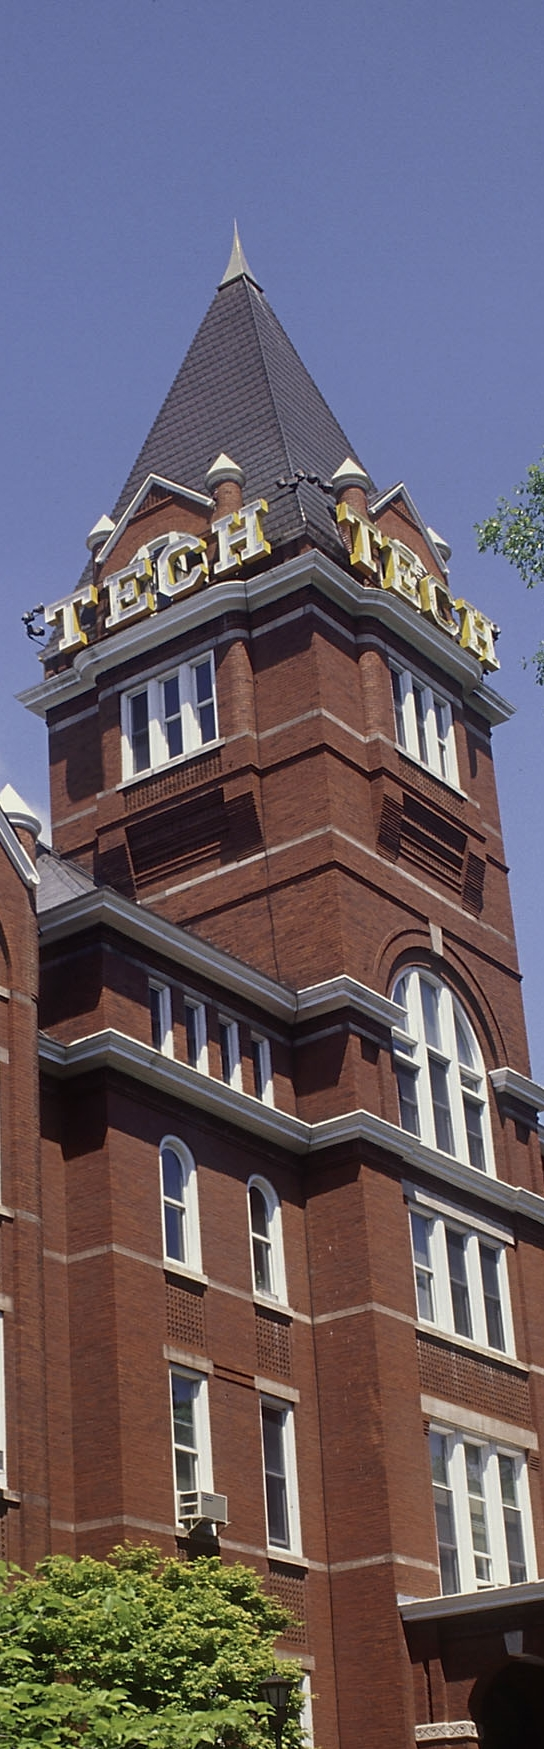
\includegraphics[width=1.25in]{figs/logo_TechTower.jpg}
    	\end{textblock}
    }

%logo tree
    \newcommand{\logoTree}
    {
    	\begin{textblock}{1}(0,0) 
    		\includegraphics[width=1.25in]{figs/logo_tree.jpg}
    	\end{textblock}
    }
%page numbers
    \newcommand{\mypagenum}
    {
    	\begin{textblock}{1}(1,94) 
		{\tiny \color[rgb]{0.2,0.2,1}\insertframenumber} %\insertframenumber,\insertpresentationendpage, \inserttotalframenumber
    	\end{textblock}
    }
%my footnote citation
	\newcommand{\myFootnoteCitation}[2]
	{
		\footnote{\tiny \citeauthor{#1}, \emph{#2}, \citeyear{#1}.}  %\citeauthor{#1}, \citetitle{#1}, #2 \citeyear{#1}.
	}
%my refer to citation
	\newcommand{\mycite}[1]
	{
		\emph{\citeauthor{#1} (\citeyear{#1})}
	}
%my footnote website citation
	\newcommand{\myFootnoteWebsiteCitation}[1]
	{
		\footnote{\tiny \citeauthor{#1}}
	}

\let\thefootnote\relax\footnotetext{Footnotetext without footnote mark}


%section underline
%\newcommand{\tmpsection}[1]{}
%\let\tmpsection=\section
%\renewcommand{\section}[1]{\tmpsection{\underline{#1}}}



%commands
	\newcommand{\likelihood}{p(Z_k| x_k) }						%likelihood
	\newcommand{\prior}{p(x_k)  } 								%prior
	\newcommand{\posterior} {p(x_k| Z_k)}						%posterior
	\newcommand{\prediction} {p(x_k| Z_{k-1})}					%prediction
	\newcommand{\update} {p(x_k|Z_k)}							%update
	\newcommand{\observations} {p(Z_k)}						%observations
	\newcommand{\prevobservations} {p(Z_{k-1})}				%previous observations
	\newcommand{\dxpk} {dx_{k-1}}							%dx_{k-1}
	\newcommand{\ChapKolm}{\int{p(x_k| x_{k-1})p(x_{k-1}|Z_{k-1})} \dxpk} %Chapman Kolmogorov

	%algorithm specific: JPDAF
	\newcommand{\likelihoodJPDAF}{p(Z_k| \chi, m, Z_{k-1}) }		%1. likelihood
	\newcommand{\priorJPDAF}{p(\chi|m, Z^{k-1}} 				%2. prior	
	\newcommand{\observationsJPDAF} {p(Z_k}					%3. observations
	\newcommand{\posteriorJPDAF} {p(\chi| Z_k)}					%4. posterior

%environments
	\newenvironment{changemargin}[2]
	{
	  	\begin{list}{}
		{
			\setlength{\topsep}{0pt}%
			\setlength{\leftmargin}{#1}%
			\setlength{\rightmargin}{#2}%
			\setlength{\listparindent}{\parindent}%
			\setlength{\itemindent}{\parindent}%
			\setlength{\parsep}{\parskip}%
		}
	  	\item[]
		}
		{\end{list}
	}
%figures

%colors
\definecolor{darkgreen}{rgb}{0,0.5,0}

%personal details
	\author{Salman Aslam}
	\institute{Advisor, Dr Christopher Barnes (ECE)\\Co-advisor, Dr Aaron Bobick (CoC)\\Georgia Institute of Technology}
	\date{}

\begin{document}
%####################################################################################################
\title{Visual Tracking \\ (shape)}
%####################################################################################################
\begin{frame}[plain]\logoTechTower
	\titlepage
\end{frame}

\begin{frame}
\frametitle{Outline}
\logoCSIPCPL\logoTechTower
	\setcounter{tocdepth}{1}	
	\tableofcontents
\end{frame}

%#######################################################################
\section{INTRODUCTION}
%#######################################################################

%==============================================================
\subsection{contour representation}
%==============================================================
\begin{frame}
\frametitle{Introduction}
\framesubtitle{contour representation: polynomials}
\logoCSIPCPL\mypagenum
	\begin{figure}
		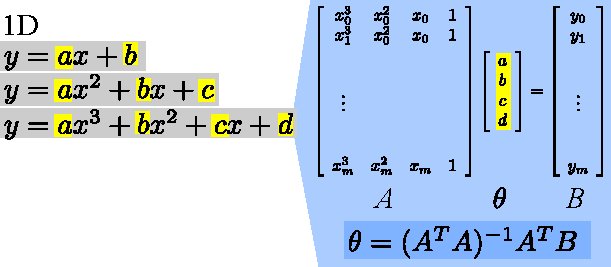
\includegraphics[width=1.0\textwidth]{figs/theory_curves_PolynomialFitting.pdf}
	\end{figure}
\end{frame}



\begin{frame}
\frametitle{Introduction}
\framesubtitle{contour representation: polynomials (cont.)}
\logoCSIPCPL\mypagenum
	\begin{itemize}
		\item convenient because they can be differentiated and integrated to get polynomials again
		\item linear, quadratic, cubic, etc
		\item possible oscillatory behavior
		\item Carl Runge demonstrated the maximum error can approach $\infty$ as number of data points approaches $\infty$
	\end{itemize}
\end{frame}




\begin{frame}
\frametitle{Introduction}
\framesubtitle{contour representation: elliptical fourier descriptors}
\mypagenum
	\begin{figure}
		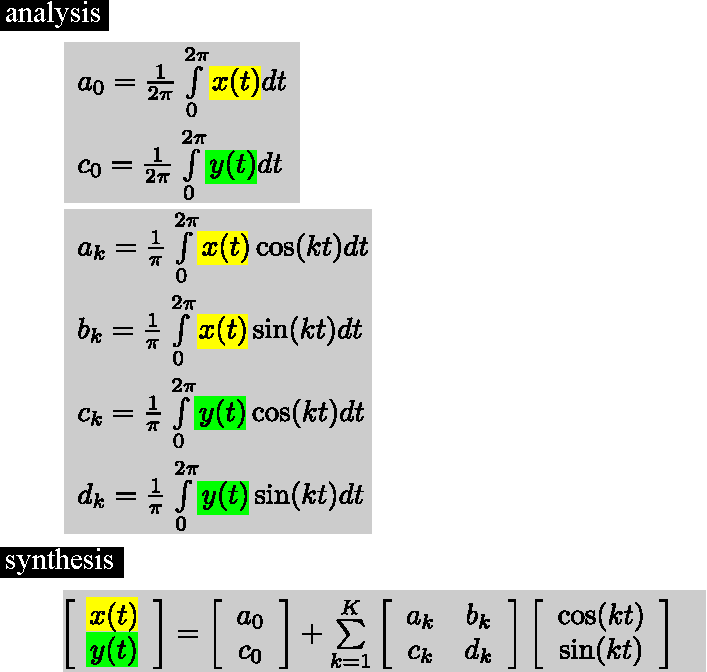
\includegraphics[height=0.8\textheight]{figs/theory_curves_ellipticalFourier.pdf}
	\end{figure}
\end{frame}



\begin{frame}
\frametitle{Introduction}
\framesubtitle{contour representation: elliptical fourier descriptors (cont.)}
\mypagenum
	\begin{itemize}
		\item extremely deformable
		\item no prior information
		\item relation between shape and parameters not clear
	\end{itemize}
\end{frame}


\begin{frame}
\frametitle{Introduction}
\framesubtitle{contour representation: splines}
\logoCSIPCPL\mypagenum
	\begin{itemize}
		\item piece-wise polynomials
		\item use $n$ low degree concatenated polynomial segments rather than a single high degree polynomial
		\item joined together at \emph{breakpoints}
		\item quadratic, order $d=3$, degree=2
		\item cubic, order $d=4$, degree=3
		\item useful when prior on shape not available
	\end{itemize}
\end{frame}



\begin{frame}[plain]
\frametitle{Introduction}
\framesubtitle{contour representation: splines (cont.)}
\mypagenum
	\begin{changemargin}{-1.3in}{0in} 
		\begin{figure}
			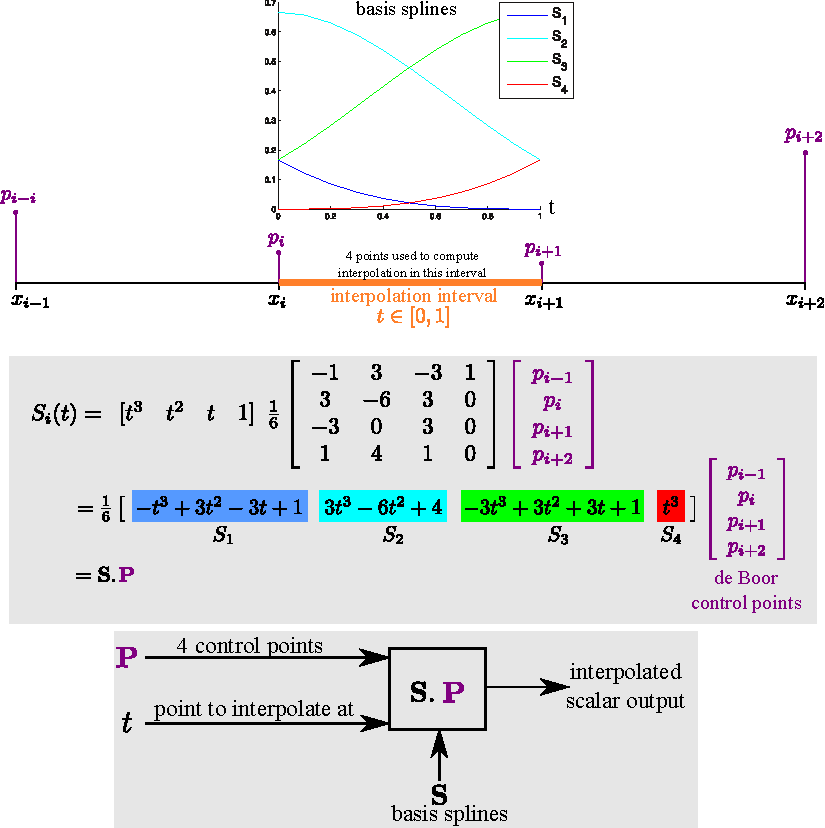
\includegraphics[height=0.85\textheight]{figs/theory_curves_UniformCubicBsplines.pdf}
		\end{figure}
	\end{changemargin}
\end{frame}

%==============================================================
\subsection{contour evolution}
%==============================================================
\begin{frame}
\frametitle{Introduction}
\framesubtitle{contour evolution: energy minimization}
\logoCSIPCPL\mypagenum
	%\begin{itemize}
	%	\item Even though the curve has corners, the first derivative remains small
	%\end{itemize}
	\begin{figure}
		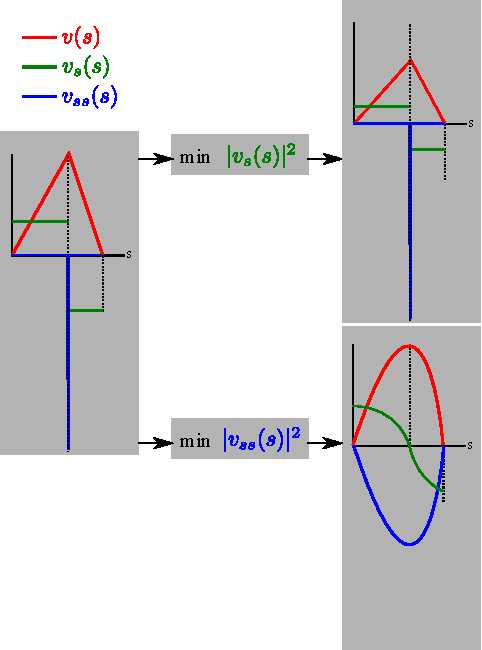
\includegraphics[height=0.8\textheight]{figs/TRK_contours.pdf}
	\end{figure}
\end{frame}


\begin{frame}
\frametitle{Introduction}
\framesubtitle{contour evolution: snakes}
\logoCSIPCPL\mypagenum
	\begin{itemize}
		\item Setting $\beta(s)$ to 0 at a point allows the snake
			\begin{itemize}
				\item to become second-order discontinuous
				\item develop a corner
			\end{itemize}
	\end{itemize}
	\begin{figure}
		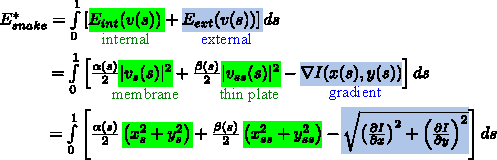
\includegraphics[width=1.0\textwidth]{figs/theory_curves_snakes.pdf}
	\end{figure}
\end{frame}


\begin{frame}
\frametitle{Introduction}
\framesubtitle{contour evolution: snakes with elliptical fourier representation}
\mypagenum
	\begin{figure}
		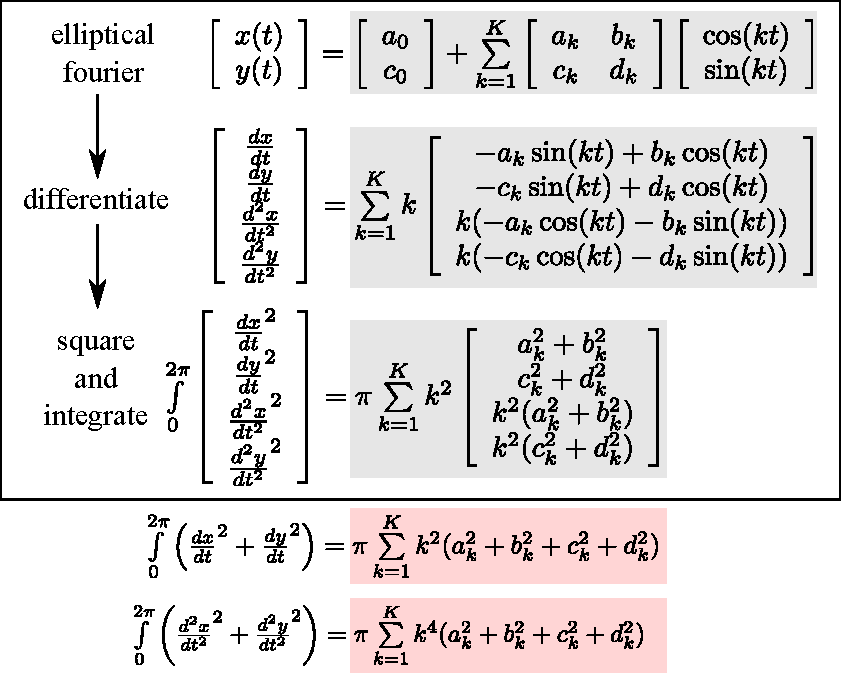
\includegraphics[width=1.0\textwidth]{figs/theory_curves_ellipticalFourierSnakes.pdf}
	\end{figure}
\end{frame}




\begin{frame}
\frametitle{Introduction}
\framesubtitle{contour evolution: snakes with elliptical fourier representation (cont.)}
\mypagenum
	\begin{figure}
		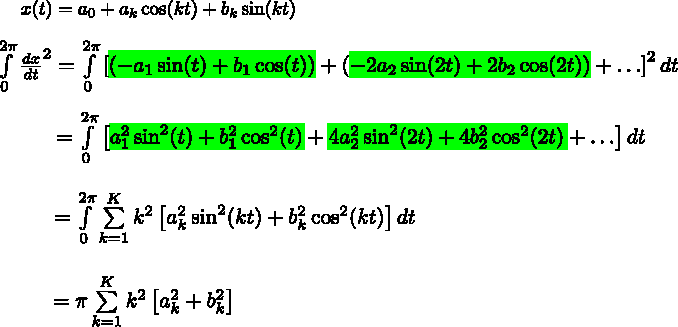
\includegraphics[width=1.0\textwidth]{figs/theory_curves_ellipticalFourierSnakes_extra.pdf}
	\end{figure}
\end{frame}



%==============================================================
\subsection{active shape models}
%==============================================================
\begin{frame}
\frametitle{Introduction}
\framesubtitle{active shape models: overview}
\logoCSIPCPL\mypagenum
\myFootnoteCitation{2000_BOOK_ActiveVision_Blake}{\emph{Active Vision}, Springer Books}
	\begin{enumerate}\small
		\item {\color{red} snakes}
			\begin{itemize}\small
				\item use prior knowledge for low-level image interpretation
				\item rather than expecting desirable properties such as continuity and smoothness to emerge from image data, these properties are imposed from the start
				\item specifically, an {\color{blue}elastic model of a continuous, flexible curve} is imposed upon and matched to an image
			\end{itemize}
		\item {\color{red} deformable templates}
			\begin{itemize}\small
				\item prior modeling can be made more specific by constructing {\color{blue}assemblies of flexible curves} in which a set of parameters controls kinematic variables
				\item a powerful mechanism for locating structures in an image
			\end{itemize}
		\item {\color{red} dynamic contours}
			\begin{itemize}\small
				\item {\color{blue}curve trackers that use prior dynamical models}
			\end{itemize}
	\end{enumerate}
\end{frame}


%#######################################################################
\section{PRIOR WORK}
%#######################################################################



%=================================
\subsection{1994: model based recognition} 
%=================================
\begin{frame}
\frametitle{Prior work: human model}
\framesubtitle{1. overview}
\logoCSIPCPL\mypagenum
\myFootnoteCitation{1994_JNL_Recog_shape_Rohr}{IU}
	%\begin{figure}
	%	\includegraphics[width=1.0\textwidth]{tables/TrackingPapers_SubspaceTracking_2006_PCA_Hog.pdf}
	%\end{figure}
\end{frame}


%=================================
\subsection{2000: W4 (Haritaoglu)}
%=================================
\begin{frame}
\frametitle{Prior work: W4}
\framesubtitle{1. overview}
\logoCSIPCPL\mypagenum
\myFootnoteCitation{2000_JNL_W4_Haritaoglu}{PAMI}
	%\begin{figure}
	%	\includegraphics[width=1.0\textwidth]{tables/TrackingPapers_SubspaceTracking_2006_PCA_Hog.pdf}
	%\end{figure}
\end{frame}



\begin{frame}
\frametitle{Prior work: W4}
\framesubtitle{2. summary}
\logoCSIPCPL\mypagenum
\myFootnoteCitation{2000_JNL_W4_Haritaoglu}{PAMI}
	\begin{itemize}
		\item static shape model
	\end{itemize}
\end{frame}




\begin{frame}
\frametitle{Prior work: W4}
\framesubtitle{figures}
\mypagenum
\myFootnoteCitation{2000_JNL_W4_Haritaoglu}{PAMI}
	\begin{figure}
		\includegraphics[width=1.0\textwidth]{figs/TrackingPapers_pedestrianTracking_2000_Haritaoglu_fig1.jpg}
	\end{figure}
\end{frame}
%=================================
\subsection{2004: crowded (Zhao)}
%=================================
\begin{frame}
\frametitle{Prior work: crowded (Zhao)}
\framesubtitle{1. overview}
\logoCSIPCPL\mypagenum
\myFootnoteCitation{2004_JNL_TRK_shape_Zhao}{PAMI}
	%\begin{figure}
	%	\includegraphics[width=1.0\textwidth]{tables/TrackingPapers_SubspaceTracking_2006_PCA_Hog.pdf}
	%\end{figure}
\end{frame}




\begin{frame}
\frametitle{Prior work: crowded (Zhao)}
\framesubtitle{2. summary}
\logoCSIPCPL\mypagenum
\myFootnoteCitation{2004_JNL_TRK_shape_Zhao}{PAMI}
	\begin{itemize}
		\item prior locomotion model to assist posture estimation
	\end{itemize}
\end{frame}



\begin{frame}
\frametitle{Prior work: crowded (Zhao)}
\framesubtitle{3. comparison}
\logoCSIPCPL\mypagenum	
\myFootnoteCitation{2004_JNL_TRK_shape_Zhao}{PAMI}	
	\begin{itemize}
		\item difficulties with blob-based analysis (see pg \pageref{fig:1})
			\begin{enumerate}
				\item a single blob may contain multiple humans due to their physical proximity or due to camera viewing angle
				\item a single object may be fragmented into several blobs due to low color contrast 
				\item blobs may contain pixels corresponding to shadows or reflections
			\end{enumerate}
				\item blobs may go through frequent structural changes (split and merge) due to above problems
				\item this causes combinatorial search for temporal correspondence
				\item even if correspondence is established, what each trajectory corresponds to (e.g. object, part of an object, a few objects together) is still unknown
	\end{itemize}
\end{frame}




\begin{frame}
\frametitle{Prior work: crowded (Zhao)}
\framesubtitle{3. comparison (cont.)}
\logoCSIPCPL\mypagenum	
\myFootnoteCitation{2004_JNL_TRK_shape_Zhao}{PAMI}
	\begin{itemize}
		\item advantages of shape based approach used
			\begin{enumerate}
				\item detecting individual objects is a goal
				\item real entities do not undergo structural changes such as split and merge
				\item constraints on (e.g. shape, size, motion) can assist segmentation and tracking
				\item less sensitive to noise and parameters of low-level processing
				\item a camera model provides additional constraints
			\end{enumerate}
	\end{itemize}
\end{frame}


\begin{frame}
\frametitle{Prior work: crowded (Zhao)}
\framesubtitle{4. contributions}
\logoCSIPCPL\mypagenum
\myFootnoteCitation{2004_JNL_TRK_shape_Zhao}{PAMI}
\end{frame}


\begin{frame}
\frametitle{Prior work: crowded (Zhao)}
\framesubtitle{5. methodology: overview}
\logoCSIPCPL\mypagenum
\myFootnoteCitation{2004_JNL_TRK_shape_Zhao}{PAMI}
	\begin{enumerate}
		\item change detection
		\item human hypotheses are computed by boundary and shape analysis using human shape and camera model
		\item each hypothesis is tracked in 3D in the subsequent frames with a Kalman filter using the object's appearance constrained by its shape
		\item 2D positions are mapped onto the 3D ground plane and trajectories are formed and filtered in 3D
	\end{enumerate}
\end{frame}



\begin{frame}
\frametitle{Prior work: crowded (Zhao)}
\framesubtitle{5. methodology: detailed}
\logoCSIPCPL\mypagenum
\myFootnoteCitation{2004_JNL_TRK_shape_Zhao}{PAMI}
	\begin{enumerate}\setcounter{enumi}{0}
		\item change detection
			\begin{itemize}
				\item single gaussian like Pfinder
			\end{itemize}
		\item camera model
			\begin{itemize}
				\item linear calibration method (\mycite{2002_BOOK_CV_Forsyth}, \mycite{1999_CNF_ModelFromIMG_Liebowitz})
				\item self calibration from walking human (\mycite{2006_JNL_Camera_Lv})
			\end{itemize}
	\end{enumerate}
\end{frame}




\begin{frame}
\frametitle{Prior work: crowded (Zhao)}
\framesubtitle{figures}
\mypagenum
\myFootnoteCitation{2004_JNL_TRK_shape_Zhao}{PAMI}
	\begin{figure}
		\includegraphics[width=1.0\textwidth]{figs/TrackingPapers_shape_2004_Zhao_fig1.jpg}
		\label{fig:1}
	\end{figure}
\end{frame}



\begin{frame}
\frametitle{Prior work: crowded (Zhao)}
\framesubtitle{figures (cont.)}
\mypagenum
\myFootnoteCitation{2004_JNL_TRK_shape_Zhao}{PAMI}
	\begin{figure}
		\includegraphics[width=1.0\textwidth]{figs/TrackingPapers_shape_2004_Zhao_fig6.jpg}
	\end{figure}
\end{frame}
%=================================
\subsection{2005: block tracking (Hari)}
%=================================
\begin{frame}
\frametitle{Prior work: block tracking (Hari)}
\framesubtitle{summary}
\mypagenum
\myFootnoteCitation{2005_JNL_TRKblk_Hari}{Trans. MM}
	\begin{itemize}
		\item according to this paper, {\color{red}motion tracking using block motion vectors has seldom been exploited}
		\item automatic initialization: skin model
		\item occlusion detection
		\item first, uncovered regions are estimated
	\end{itemize}
\end{frame}










%####################################################################################################
\section{METHODOLOGY}
%####################################################################################################
\begin{frame}
\frametitle{Methodology}
\framesubtitle{steps}
\logoCSIPCPL\mypagenum
	\begin{enumerate}
		\item Parameterize curve to get shape parameter $\mathbf{x}$
			\begin{itemize}
				\item example, use B-spline curves
				\item control points could be used, but this would allow too many degrees of freedom
				\item create shape space
			\end{itemize}
		\item Predict: Markov-chain model in shape space
		\item Update: Fuse information from prediction and observation
	\end{enumerate}
\end{frame}



%####################################################################################################
\printbibliography
%####################################################################################################
%\bibliographystyle{ieee}
%\bibliography{c:/salman/work/writing/MyCitations}
\end{document}
%####################################################################################################

%####################################################################################################
